% --------------------------------------
% Master's Thesis Title Page
% LaTeX Template
% Version 1.0 (23/05/14)
% Thanks to Magnus Marthinsen, this thesis and template is made available for Master studentes at HVL Joint SE program (01.03.2021)
%---------------------------------------

%----------------------------------------------------------------------------------------
%	PACKAGES AND OTHER DOCUMENT CONFIGURATIONS
%----------------------------------------------------------------------------------------
\documentclass[a4paper]{report}
\usepackage{graphicx} % Required for box manipulation
\usepackage{helvet}
\usepackage{subfig}
\usepackage[utf8]{inputenc}
%\usepackage{natbib}
\usepackage[USenglish]{babel}
\usepackage[useregional]{datetime2}
\usepackage{pgfgantt}
\usepackage{listings}
\usepackage{wrapfig}
\usepackage{setspace}
\usepackage{parskip} % Used to create spaces between paragraphs
\usepackage{dirtytalk} % quotes by talk
\usepackage[hidelinks]{hyperref}
% \usepackage[acronym, toc]{glossaries}  % Used to add a wordlist/glossaries
\usepackage{mathtools}
\usepackage{amsfonts}
\usepackage{color, colortbl}
\usepackage{booktabs}
\usepackage{float}
\usepackage{csquotes}

%BIB by Adrian
\usepackage[backend=biber,style=numeric, urldate=long]{biblatex}
% See the references.bib file. Most Bibtex bibliographies in Computer Science can be found from dblp.org
\addbibresource{report.bib}



% Glossary/wordlist
% \makeglossaries
% \input{glossaries.tex}

\begin{document}

%
% COLORS USED THROUGH THE REPORT
%
\definecolor{kb_red}{RGB}{96,2,4}
\definecolor{light_gray}{RGB}{160,160,160}
\definecolor{med_gray}{RGB}{96,94,94}
\definecolor{black}{RGB}{0,0,0}
\definecolor{white}{RGB}{155,155,155}
\definecolor{light_green}{RGB}{208,240,192}
\definecolor{light_red}{RGB}{255,204,203}

% CODE STYLE
\definecolor{javared}{rgb}{0.6,0,0} % for strings
\definecolor{javagreen}{rgb}{0.25,0.5,0.35} % comments
\definecolor{javapurple}{rgb}{0.5,0,0.35} % keywords
\definecolor{javadocblue}{rgb}{0.25,0.35,0.75} % javadoc

\makeatletter
\lst@Key{matchrangestart}{f}{\lstKV@SetIf{#1}\lst@ifmatchrangestart}
\def\lst@SkipToFirst{%
    \lst@ifmatchrangestart\c@lstnumber=\numexpr-1+\lst@firstline\fi
    \ifnum \lst@lineno<\lst@firstline
        \def\lst@next{\lst@BeginDropInput\lst@Pmode
        \lst@Let{13}\lst@MSkipToFirst
        \lst@Let{10}\lst@MSkipToFirst}%
        \expandafter\lst@next
    \else
        \expandafter\lst@BOLGobble
    \fi}
\makeatother

\lstset{language=Java,
basicstyle=\footnotesize,
keywordstyle=\color{javapurple}\bfseries,
stringstyle=\color{javared},
commentstyle=\color{javagreen},
morecomment=[s][\color{javadocblue}]{/**}{*/},
numbers=left,
captionpos=b,
frame=single,
breakatwhitespace=false,
breaklines=true,
numberstyle=\tiny\color{black},
stepnumber=1,
numbersep=10pt,
tabsize=2,
showspaces=false,
showstringspaces=false,
matchrangestart=t}

%----------------------------------------------------------------------------------------
%	TITLE PAGE
%----------------------------------------------------------------------------------------

\newcommand*{\titlePage}{\begingroup % Create the command for including the title page in the document
\fontfamily{phv}\selectfont
\centering % Center all text
\DTMlangsetup[en-US]{showdayofmonth=false}

%----------------------------------------------------------------------------------------
%	TITLE SECTION
%----------------------------------------------------------------------------------------

\vspace{200pt}
{\Huge VR viewer} \\ % Title
\vspace{5pt}

{\Large \textsl{}} % Subtitle or further description
\vspace{50pt}

%----------------------------------------------------------------------------------------
%	AUTHOR SECTION
%----------------------------------------------------------------------------------------

\LARGE{\textbf{Tobias Eilertsen}}\\ % Author name

\vfill % Whitespace between the author name and the school

%----------------------------------------------------------------------------------------
%	DESCRIPTION AND DATE SECTION
%----------------------------------------------------------------------------------------


{\Large \textbf{Master's thesis in Software Engineering at} \\
\vspace{10pt}
Department of Computer science, Electrical engineering and Mathematical sciences, \\
Western Norway University of Applied Sciences \\
\vspace{10pt}
Department of  Informatics, \\
University of Bergen \\}
\vspace{10pt}
{\large \today} % Month and year published

%----------------------------------------------------------------------------------------
%	LOGO SECTION
%----------------------------------------------------------------------------------------

\vfill % Whitespace between the school and the publisher logo


\begin{figure}[h!]
	\captionsetup[subfigure]{labelformat=empty}
	\subfloat[][]{
\includegraphics[height=70pt]{images/logos/hvl_logo_engelsk.pdf}}
	\hfill
	\subfloat[][]{
\includegraphics[height=70pt]{images/logos/uib-logo.eps}}
\end{figure}


\endgroup}

\titlePage
\pagebreak

\section*{Abstract}
During the planning of a surgery in orthopedics, the surgeons will use CT scans and sometimes 3D printing to analyze the fracture and help prepare for the surgery. By using Virtual Reality technology, the data can be visualized in 3D in a more immersive way, potentially improving the preparation phase by increasing the anatomical understanding or removing the need for 3D printing.

% \section*{Acknowledgements}
% First and foremost, I would like to thank

\pagebreak
\tableofcontents
\listoffigures
% \listoftables

% \printglossary[nonumberlist]
% \printglossary[type=\acronymtype, nonumberlist]

\chapter{Introduction}
This thesis is written as part of the University of Bergen and Western University of Applied Sciences master programme in software engineering. The project is a collaboration with Helse Vest IKT and orthopedic surgeons at Haukeland University Hospital.


\section{Context and Approach}
A CT scan is often performed when a hospital receives an injured patient considered for orthopedic surgery. The CT scan is displayed as 2D images or as a 3D model. The model allows the surgeons to better plan the surgery by understanding the anatomy of the fracture.
If a surgeon has a good understanding of the anatomy related to the fracture,
the surgery has less risk of complications or could require fewer resources.

\section{Problem Description}
Visualizing the model in 2D limits the understanding of the fracture because of the lack of scale and depth. The problem applies to both 2D images and 3D models rendered in 3D.
A considered solution is visualizing the model in Augmented Reality or Virtual Reality to give medical personnel a good understanding of the problem area.
VR has multiple potential benefits, and the surgery planning process can use some of these. As the users are already looking at 3D models on 2D screens, visualizing in VR could improve the surgeon's overview and patient safety. The entire planning process could also be more effective by removing or reducing the need for 3D printed models, especially in cases with limited time. Therefore the possible research questions are as follows:

How can VR technology improve surgery planning by

1: a better understanding leading to a better success rate.

2: replacing 3D printing while using less resources or time.

\section{Methodology}

The project should include a VR prototype of a standard where it is
user friendly enough to test with non-technical subjects and with functionality
that is comparable to the use cases of a printed model.
The prototype is tested on medical personnel to measure any benefits on anatomical understanding and how it affects surgery planning and effectiveness.
The application should be available for further development and study.

Firstly, a prototype VR viewer will be created with the help of related
open-source frameworks/software and guidance from both orthopedic surgeons and
developers with experience in medical technology.

In order to answer the research question, we will measure the
usability of the final application. This thesis will use qualitative methods
by interviewing related personnel to investigate the performance, including
anatomical understanding, cooperation, and the effectiveness of the planning
process.
The performance will also be put in context to the existing solutions, possibly
by making a direct comparison by using a 3D model, printed model, and VR viewer
on the same case.

\section{Related works}

There currently exists several alternatives to viewing medical data in VR, here are some of the alternatives:

Medical Holodeck~\cite{medical_holodeck_medicalholodeck_nodate} $Medical imaging XR$ is made for surgeons to plan surgeries and medical education.

An Augmented reality viewer called Dicom Director also exists, and is not yet approved for clinical use.\cite{dicomdirectorcom_surgeons_nodate}

Other similar solutions are Materialise\cite{materialise_medical_nodate} and
Ceevra\cite{ceevra_inc_using_2019}.

Most current solutions are closed source premium services targeted at enterprise/medical institutions. Many of them are not yet approved for clinical use, and current solutions are difficult to use for people not used to Virtual Reality \emph{cite Håkon?}

Some free general purpose VR viewers for 3D models also exist, but I have not found any with features related to medical use, collaboration or planning. Importing DICOM data is also not supported.

A study in visualising Patient data with VR\cite{vertemati_virtual_2019} implemented a VR viewer for DICOM data and tried to measure anatomical understanding compared to 2D images. The study did not investigate the efficiency of the planning phase, and it did not consider 3D printing.

\section{Contribution}
\section{Outline}

\chapter{Background}\label{Background}
This chapter will present some of the knowledge that our research is built upon. 

\section{orthopedic surgery}

Orthopedic surgery is surgery involving the musculoskeletal system. Cases range from trauma surgery, where high impact forces cause injuries to infections and tumors\cite{manual ortho}.

Orthopedic surgeons do both elective (planned) and urgent surgery. In elective surgery, the surgeons will have days or weeks to plan out the surgery. A team of usually two surgeons will plan the surgery together.
A surgeon will diagnose the patient from the following features: history, clinical examination, medical imaging, and any special investigations. History includes the patient's complaint and any previous injuries. Clinical investigation means examining the sources of the symptoms and the body as a whole. Medical imaging, including ultrasound, CT, and MRI, gives the surgeons a detailed insight into bones or soft tissue structures.

This research is based on elective surgeries on trauma or fractures where the surgeons plan out the surgery with different tools.

\subsection{surgery types}
--what makes surgery complicated
--perkutant
--ledd
--viktig å reponere eksakt pga slitasje
-- eks calaneus

\subsection{Brief history of medical imaging}
The first used imaging tool was the X-Ray, discovered in 1895\cite{hamblen_outline_2010}\cite{suetens_fundamentals_2017}. As the energy in the radiation is absorbed at a different rate by tissue and bone mass, it is possible to create an image of the bone. The image is displayed as a projection from the X-ray angle. During the first half of the 20th century, additional techniques with several X-Rays allowed to isolate a slice of bone without over- and underlying tissue. A big leap in medical imaging was the CT scan (computed tomography)\cite{bradley_history_2008}
CT scans (Computed Tomography) were invented during the 1970s. During a CT scan, an X-ray tube is rotated around the tissue, scanning from all angles while detecting the absorption/reflection of the tissue. CT scans overcome the two-dimensional X-ray limits and create detailed image data that can be visualized in any plane without superimposing the image with tissue above and below the selected layer\cite{hamblen_outline_2010}. The detail of a CT scan depends on the hardware used, as well as the trade-off where higher resolution gives the patient higher radiation\cite{bradley_history_2008}. CT scans can eliminate the need for repeated imaging in the case of a trauma patient\cite{swiontkowski_manual_2013}.
MRI (Magnetic Resonance Imaging) was also developed during the 70s. It uses a strong magnetic field and radio signal frequencies to scan. MRI has better accuracy than CT when measuring soft tissue and avoids radiation.


The imaging used for testing in this report is from CT scans done by Helse Vest.

\subsection{Visualisation of medical imaging}

\begin{figure}[h!]
    \centering
	\subfloat[][]{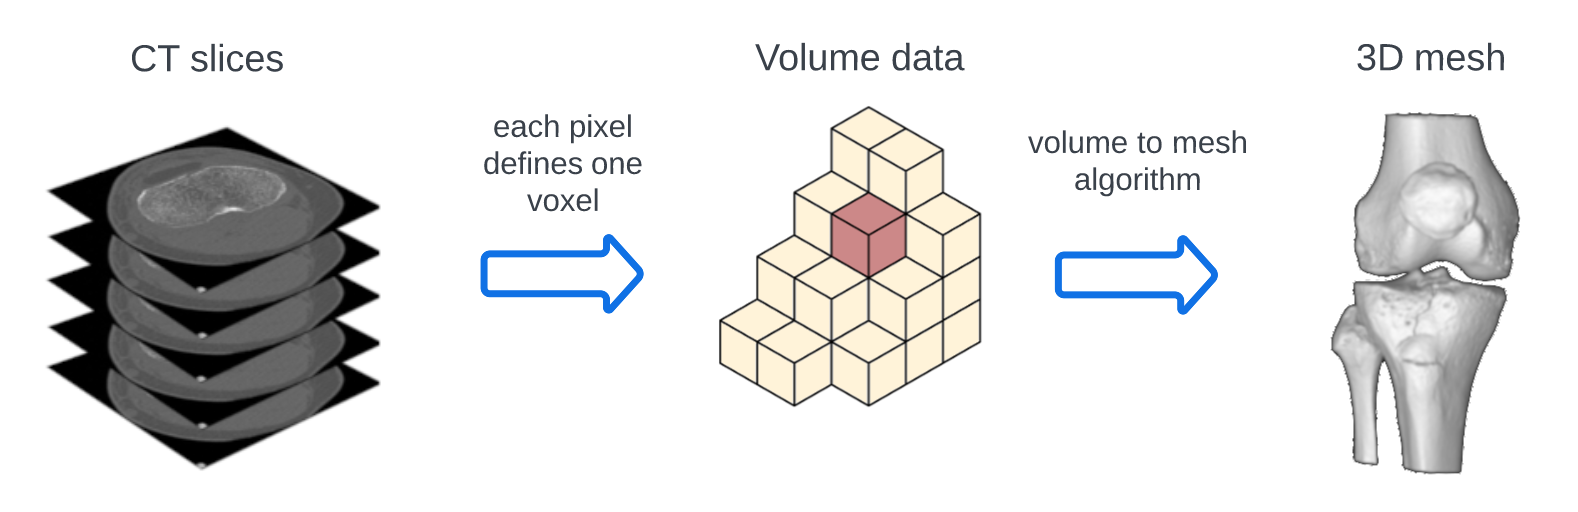
\includegraphics[height=120pt]{images/slices.png}}
	\hfill
  \caption{Transforming DICOM data into a polygon mesh}
\end{figure}

The output of both CT and MRI scans is a three-dimensional scan. The output is typically represented as slices, where a slice is a 2D picture repeating along an angle. The pixel at coordinate \emph{(x, y)} at slice number \emph{z} represent the absorption at the point \emph{(x, y, z)}\cite{chougule_conversions_2013}.
Each pixel in a slice represents a voxel in a volume, and all the slices combined make up volumetric data or a three-dimensional point cloud\cite{chougule_conversions_2013}.
The slice thickness of a slice can be below 1 mm, giving a high-resolution scan where a single point is less than one cubic millimeter\cite{hamblen_outline_2010}.

When rendering a 2D image, the volume must be projected to two-dimensional space. The values in a single slice can be used to view the intersection at a specific slice number. A line of values along all the slices can be used to view the intersection at another plane.
All slices can be combined to show either the average or the maximum intensity\cite{fishman_volume_2006}.
The values are converted to greyscale by mapping ranges of values to greyscale pixels. This mapping function determines the brightness and contrast of the final image.

A specific algorithm is needed to render the scan as a 3D surface mesh. Rendering the model includes preprocessing the volume and classification to determine the type of tissue based on voxel value. A simple approach is thresholding, a binary classification where a polygon is created on any volume point that matches the threshold value. A different threshold can be selected to visualize tissue with different densities, typically bone\cite{fishman_volume_2006}.

\subsubsection{ 3D printing }

\begin{figure}[h!]
    \centering
	\subfloat[][]{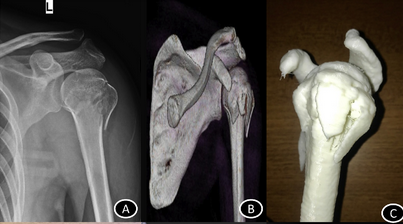
\includegraphics[height=120pt]{images/ctToPrint.png}}
	\hfill
  \caption{Humeral (upper arm) fracture}
  \small
    A fracture from initial scan to finished print. (A) preoperative X-ray; (B) 3D model; (C) 3D printed model.
~Image from study on virtual preoperative planning~\cite{mishra_virtual_2019}
\end{figure}


An alternative to digital representation is to print the model with a 3D printer. 3D printing has many advantages, such as the surgeon physically holding the model, measuring the model, trying out equipment, and practicing with the model.
The most significant disadvantage to 3D printing is that the printing process can take more than 24 hours depending on model size, materials and printer. This is in some cases too long. Another drawback is not having any digital tools such as transparency, displaying cross-sections, or being able to alter the model in any way. A physical plastic model also needs support structures that can lead to an inaccurate representation of the fracture or get in the way of viewing the model.

TODO: cost, resources?

A possible use case for a VR viewer is inspecting a fracture in VR and then deciding if a printed model is necessary, to avoid spending time on an unnecessary printing process.

\section{Virtual Reality}
Virtual Reality is the use of VR technology to sense the user's state and actions and augment sensory feedback to immerse the user in a 3D virtual environment\cite{mihelj_virtual_2014}.

The virtual reality system works by tricking the senses by displaying computer-generated stimuli that replace stimuli from the real world. The user typically perceives the virtual environment through a Head-mounted Display (HMD), sound, and haptic feedback (vibration). 
The virtual environment is the computer-generated objects that the user interacts with. The virtual environment will often mimic properties in the real world, such as shape, color, or functionality.

With more specialized hardware, additional stimuli such as temperature, smell, and more are possible\cite{noauthor_feelreal_nodate}.
To make the virtual environment seem real, it must respond to the user's actions. Current commercial Virtual Reality headsets track the user's head and hands and allow for button inputs\cite{noauthor_oculus_nodate}. Modern HMDs use 6 Degrees of Freedom (DOF), which means the user is tracked in three-dimensional position and rotation\cite{lang_introduction_2013}. The tracking is used by the VR application to simulate walking, picking up objects, and more.

\subsection{Professional usage of VR}
While becoming more popular in mainstream entertainment, VR has been used in professional environments for a long time\cite{needed}. VR and AR are often used in the medical field for training or education because the actual situation would be unpractical or dangerous\cite{freina_immersive_2015}.

TODO: finne kilde på remote surgery o.l.?

\subsection{Advantages and disadvantages}
A disadvantage with wearing an HMD is fatigue, both physical fatigue caused by the weight or eye fatigue and motion sickness\cite{merhi_motion_2007}.
Image imperfections cause eye fatigue in the HMD\cite{kooi_visual_2004}, and motion sickness is caused by sensory conflict.
According to a study on motion sickness factors, 59 \% of the subjects experienced motion sickness after a mean of 14 minutes. The remaining subjects did not experience any illness\cite{kooi_visual_2004}. Motion sickness can be mitigated in several ways.


A use-case of VR is simulating a subject physically out of reach, such as a planet in space or the inside of a patient's knee. For physically impaired users, this advantage is even more relevant.
VR can also simulate things that would otherwise be dangerous, for example, an untrained surgeon performing surgery alone.
Another advantage is that VR is more immersive than other mediums. The immersion makes the user feel more stress or fear and makes it feasible to prepare personnel for stressful situations, such as the police.
The added immersion also makes teaching or training more motivating for the student.\cite{freina_immersive_2015}

\subsection{ Augmented Reality }
Augmented Reality (AR) or Mixed Reality is an upgrade of VR where the real world is mixed with the virtual environment\cite{hackett_three-dimensional_2016}. AR comes in different variants; some mobile apps use the camera to create an AR environment, and AR HMDs work similarly to VR HMDs, except that the viewing glass is transparent.
AR HMDs are used in medical, industrial, and military devices to show critical information while users operate devices or perform a job in real life. Examples of this are a surgeon viewing medical information during a surgery or a pilot viewing a Heads Up Display while flying\cite{mihelj_virtual_2014}.
AR has some uses not relevant for VR because it does not completely disconnect the user from the real world, but has some disadvantages such as reduced field of view compared to VR, poor visibility in bright light\cite{hackett_three-dimensional_2016} and drastically higher cost\cite{medical_holodeck_medicalholodeck_nodate}.

\subsection{Designing for VR}
VR is relatively new to mainstream media, and as such, there are few agreed-upon standards, unlike e.g., web development.
Some effective measures to counter motion sickness and fatigue are reducing Field of View (FOV), varying latency between user input and display update, flickering, moving content in the virtual environment, using several stimuli (audio, haptics)\cite{chang_virtual_2020}. Some of these are hardware-dependent and not relevant for this project, so moving content is the most relevant measure in this project.

\subsection{Unity}

The Unity game engine is used for developing the application\cite{unity}. Using a game engine speeds up the development as it includes systems needed, like rendering, animations, and physics. Unity is widely used for game development\cite{gameenginesonsteam} and is well documented online with a lot of community-supported plugins.

Unity has good support for different VR and XR platforms\cite{unityxr} including the OpenXR standard widely used by VR headsets\cite{openxr}. This framework allows creating VR games with Unity handling most VR logic.

Part of the Unity VR support is the XR interaction Toolkit (XRTK)\cite{xrinteractiontoolkit}. It is a high-level framework for using XR interactions with unity events. The toolkit also includes components for selecting/grabbing, haptic feedback, and UI interaction.

To develop for several XR platforms, the different controllers have a mutual interface for setting keybindings, called an XR controller. Almost all commercial VR controllers support an index finger trigger, a joystick/trackpad with 2D directional input, a grip button, and at least one extra button\cite{technologies_unity_nodate}.



\chapter{Design and Implementation}\label{Design and Implementation}
TODO: flytte?
The application was developed by me in about 7 months. I have no medical experience and was supported by staff at Helse vest with guidance and expertise on orthopedics, medical imaging and Unity, and VR development.

\section{Demonstration}\label{demonstration}
gameplay

\section{Development methods}

\subsection{Research Method}
The research question is solved by developing an application, and evaluating the application with respect to the research questions. Qualitative testing is used to evaluate the application, because of a low test user amount.

The largest part of the study is developing the application that fills the need of viewing CT data. This is accomplished by uncovering user needs with interviews and user testing. When the application meets minimum specifications, an evaluation if performed. 

The evaluation at the end of the project aims to answer both research questions. The evaluation is done in the following way:
The test users try the application on their own in a relevant scenario.
The users respond to a semi-structured interview. The questions are specific towards both research questions.

The responses are gathered and used to answer the questions.

\subsection{Iterative Development}
\begin{figure}[h!]
    \centering
	\subfloat[][]{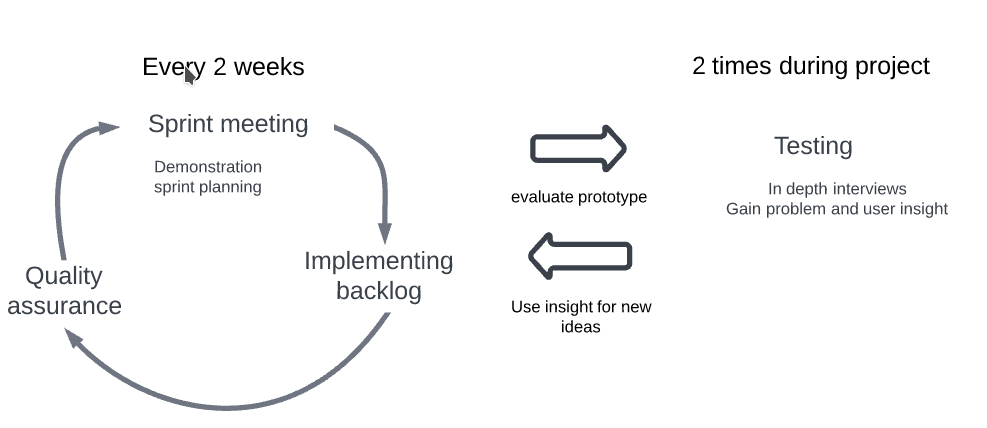
\includegraphics[height=120pt]{images/agile.png}}
	\hfill
  \caption{Development method}
  \small
  Scrum sprints illustrated on the left, and user testing on the right.
\end{figure}

The application is developed using iterative development and elements from Design Thinking and Scrum.

Scrum was used to cooperate effectively with the team and increase the development speed. The team had regular meetings and this fits well with the sprints used in scrum and the surgeon on the team was a natural product owner.
The team had regular biweekly meetings with a demonstration, sprint retrospective, and sprint planning. The Sprint meeting was a valuable way of sharing interdisciplinary information and getting feedback from medical experts. Sprint retrospective and daily scrum was not relevant as only one person worked full time on the project.
After the biweekly demo, the sprint backlog was updated with tasks prioritized by value. The value is determined by the time needed to implement compared to how important the functionality is to the medical personnel. Any tasks or ideas remaining are stored in the product backlog and considered for the next sprint.
The frequent Scrum demonstrations worked really well with VR development, as the different features are hard to understand without trying the application. Fast prototypes are important to cooperate efficiently when the product owner or test users have a limited understanding of the technology.

Design thinking was loosely used because the medical domain and user needs was difficult to understand. I specifically used the ideate, prototype and test pattern to develop the application
The application demos served as smaller user testing sessions. The medical personnel in the team would try out the application and any new features and give feedback and ideas during testing. User testing would often lead to new ideas. Optimally the test subjects should have been personnel outside the project without any bias, but busy schedules and COVID restrictions limited this.

\section{Project overview}\label{CodeStructure}

\section{Design}

\subsection{Design goals}

The goal of the application design is as follows:
give a good understanding of what the fracture looks like (bruddlinje og mindre biter)
Ease of use for non technical personnel
Be able to cooperate in smaller teams - multiplayer

\subsection{Anatomical understanding}
TODO: how to give the user a good understanding of a fracture

\subsection{VR interface}

TODO: Overview image

To make the VR interface easy to use, I focused primarily on familiarity with current tools and a simple design.
I used MicroDICOM\cite{MicroDICOM} as a reference for a familiar tool.
Familiarity with current tools means taking interactions from programs such as CT viewers and adopting the same interactions to VR to make it recognizable and consistent to the user. An example of this is navigating a menu in VR the same way one would navigate a menu with a pc mouse.
 All unnecessary interactions and information is removed to allow new users with little VR experience to start using the program quickly. The goal is to make the experience less overwhelming and lower the skill required to use the viewer effectively.

\subsubsection{Learning process}
A video game style tutorial was considered, where the user would go through tasks with hints or descriptions of the features in the application. However, this was not implemented as early testing revealed users were learning the controls quickly.

Every button has a description displayed as text above the button to remind the user of the keybindings. An image can optionally be displayed, showing the user the keybindings. The hints were implemented as users repeatedly forgot button controls in testing.

\subsubsection{Grab interaction}

The most used part of the interface is moving the fracture parts to inspect or rearrange them. The grab should mimic how users move objects in real life to make this easy to use. When the user places the hand close to a model part, the color is tinted to highlight the model. When the grab button is pressed, the highlighted model part is picked up, and a short audio clip is played.

One issue is that the user might want to move either the entire model or move a part of the model. Including both could introduce mode issues\cite{nngroup}, so the grab interaction always picks up a model part. A joystick input moves the entire model.

The grab functionality is implemented using Unity's built-in $Interactable$ system for XR\cite{noauthor_xr_nodate} development. This allows to set up grabbing, throwing, and more. 
By default, the grab will move the center of the interactable to the user's hand. The built-in grab action is cumbersome when precisely adjusting larger objects, as moving the interactable a small distance requires repositioning it from wherever the center is. 
To solve this, the interactable script is modified to keep the current position when grabbed, and then follow the relative motion of the hand.

To allow for grabbing small objects or objects that are partly overlapping, what objects are selected is also modified. The default Unity XR behaviour is selecting a new object every frame, and this would lead to the user grabbing several objects simultaneously. To solve this, any interactable is highlighted when the users hand is within the collision box. It stays highlighted until the hand is outside of the collision box. The grab action is only allowed to select the hovered object, until the grab is released.


\subsubsection{Separation mode}
The grabbing functionality introduces a problem: If the user moves a model part, the CT images will no longer be similar to the model displayed. Also, if the user is measuring the distance between two model parts, it gives an invalid result if the parts are moved. 
The solution to this is a separation mode. Moving any model part enters separation mode and reverting to the original position exits separation mode. In separation mode, the CT images are hidden, and measurements are hidden. A large button appears to display the current mode, prompting the user to click the button to reset the model and once again view CT images.

\subsubsection{Keybindings}

\begin{figure}[h!]
    \centering
	\subfloat[][]{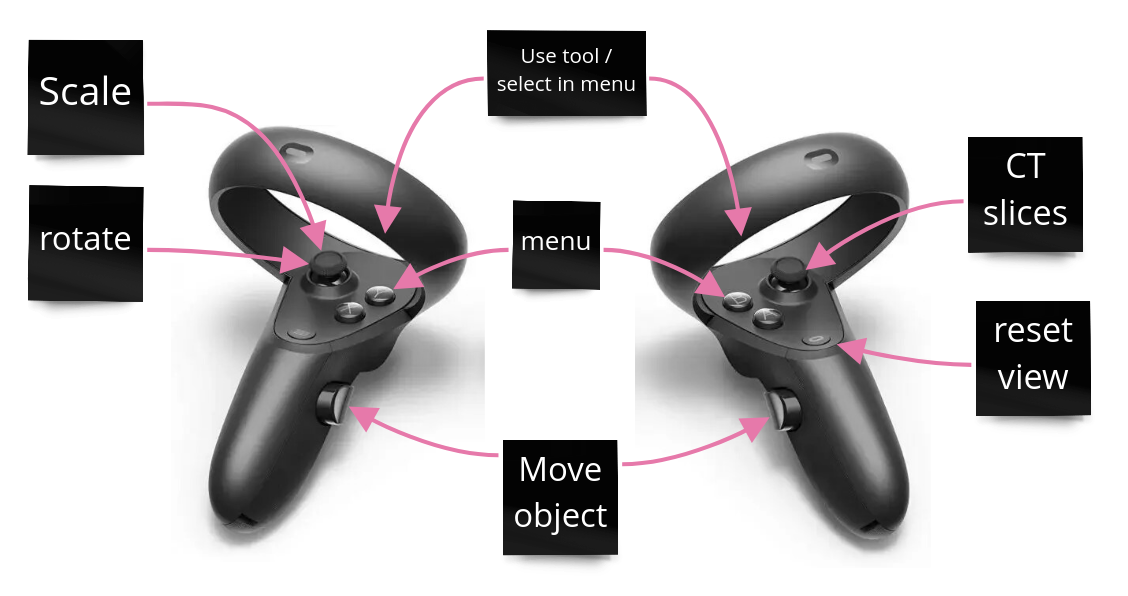
\includegraphics[height=120pt]{images/controllers.png}}
	\hfill
  \caption{Keybindings on Quest controllers}
  \small
  This illustration is also used within the application.
\end{figure}

The most common operations are bound to trigger and grip button, which is easily reachable on most controllers. The controller trigger mimics a mouse click on a pc, and so it is used for clicking buttons and using selected tools. The grip button mimics a real-world grabbing gesture and is used for grabbing a model part.
The primary button is used for opening the menu.
For ease of use, the two controllers are mostly mirrored, except for the joystick. The right joystick is used for scrolling through CT slices, similar to how the scroll wheel is used in CT image viewers. The left joystick rotates and scales the entire model while keeping all the model parts correctly positioned.

\subsubsection{Menu system}
A menu system is implemented to allow the user to navigate less common operations while not distracting from inspecting the model.
When the menu button is pressed, the menu screen appears in front of the user. It is shown in world space, which means the text appears as a physical screen. The model is temporarily hidden to ensure the menu is always in the user's field of view. Placing content at the center of the screen avoids a typical VR UX problem where some information is not visible to the user.

\begin{figure}[h!]
    \centering
	\subfloat[][]{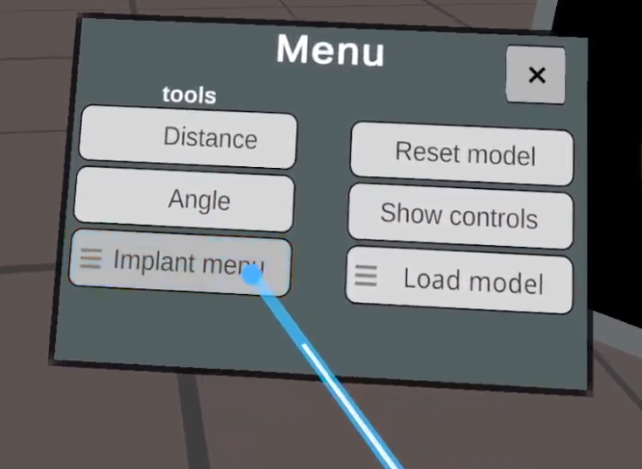
\includegraphics[height=120pt]{images/menu.png}}
	\hfill
  \caption{Menu screen}
  \small
  The main menu interface. The user is hovering one of the buttons.
\end{figure}

The menu includes access to less frequent actions that do not require their own keybinding. The initial menu includes fast access to simple tools (e.g., measurement) and buttons to sub-menus. A hamburger menu icon suggests the button leads to a sub-menu.

The menu layout consists of one or more vertical lists of buttons. Several columns of lists are used to separate buttons into categories. To keep the menu simple and consistent, only buttons are used for interacting with the menu. The 'cross' button from pc programs is used for exiting the menu.
The sub-menus are implemented when multiple options are present. It is used for selecting an implant type or loading a new dataset.

\subsubsection{Measurements}
Some important functionality available in desktop VR viewers should also be available here. This includes measurement of distance and measurement of angles.
The measure tools works by selecting a start and an end point. The angle measurement additionally requires a middle point.
After placing the first point, a preview of the measurement result is shown as a line to give feedback to the user of the current state.
Using the outline shader mentioned before makes it possible to see the placed points even when obscured by the model, and the line between the points is always visible. This, combined with depth in VR makes it easy to understand where the points are placed and what the length and angle is.

\begin{figure}[h!]
    \centering
	\subfloat[][]{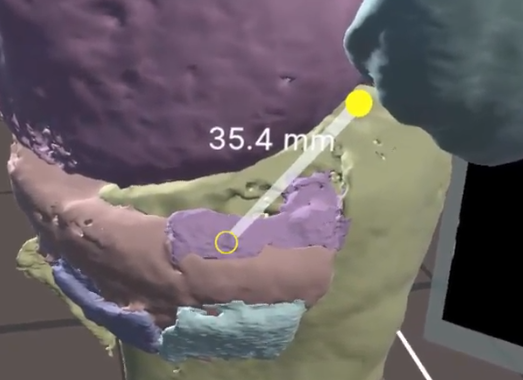
\includegraphics[height=120pt]{images/measure.png}}
	\hfill
  \caption{Distance measurement}
  \small
  A distance measurement. The yellow hollow circle is inside the model, and the filled circle is in front of the model.
~\cite{mishra_virtual_2019}
\end{figure}

\subsubsection{Audio}
Audio is mainly used for interaction feedback. If the user successfully picks up a model part, a sound is played to indicate the user is holding something.

\subsubsection{Motion sickness}
The most relevant motion sickness factor for this project is the use of motion and static content. The only moving content is the fracture model, which only moves because of player input. The environment is designed like an office room and is always static. All HUD elements are also static, with few exceptions.
During multiplayer, the model may move caused by another player's input, which might cause some motion sickness if the model is viewed by the user. This could be solved by hiding the model when it moves, but it could interfere with the multiplayer experience if the model suddenly disappears.

\subsection{Multiplayer design}
The goal of the multiplayer feature is to allow two or more surgeons to cooperate effectively. Having one surgeon using a VR headset and another using a screen is likely interfering because the surgeons are seeing different models. The multiplayer component allows the surgeons to use the same tools while seeing the same model.
Multiplayer should not make the application more difficult to use. All interactions should be similar to the usual experience, and cooperation should not require any extra steps, except connecting to the multiplayer server. Any important information should be available to all players, and irrelevant information (another player opening a menu) should not be disturbing.

The multiplayer UI is a menu shown at startup. The user can select either to start a new session in which other users can join, or join an existing session. The sessions are hardcoded to always run on the same port and have no authentication, as this would take too much development time and give no value.

\subsubsection{Mirror}
The networking was built with Mirror, a downloadable Unity asset. Mirror is a high-level networking API built on deprecated Unity networking\cite{noauthor_mirror_nodate}. Mirror has good support for creating a client/server pattern and classic video game related operations such as spawning in players at the start of the game and synchronizing objects across all clients.

\section{DICOM data visualisation}
I received several anonymized CT scan files from Helse Vest to use as input data. The CT scans are sent as DICOM packages\cite{noauthor_dicom_nodate}, where the scan is stored as several files, each representing a slice.
The model is also split up into bone fragments. The files include 3D surface models as STL files, where each file contains one bone. The STL files are created by (radiograf ???) at Haukeland University Hospital.


\subsection{Unity with custom file types}

To be able to read the DICOM files, the build produced by Unity needs access to the files. Unity has several built-in solutions to this.
The most common is the Resources functionality\cite{resourcesload_unity_nodate} that builds the application and includes all files in a `Resources' folder. Android projects are built in the standard APK format and also require special file paths and using the built-in web request to read files. This is not well documented, especially for the Quest, so this method was scrapped.

The easiest way of referencing files is usually setting a reference in the unity editor, and the file will be included in the build. This works great with common files like images, but Unity does not allow custom file types without 'hacking' the Unity inspector and creating a custom file importer\cite{scriptedimporters_unity_nodate}, that has lacking documentation. The solution to this is to rename all DICOM files to {name}.bytes. This makes Unity handle the files as 'TextAsset' text files\cite{textassets_unity_nodate}. I then open the files as text files and create a byte stream. The byte stream is then used for rendering with the DICOM library.

\subsection{Rendering CT image}
TODO: cite dat253?
TODO: begreper

To render CT images from the DICOM data, I used the .NET library \emph{Fellow Oak DICOM}\cite{noauthor_fellow_2022}. It is an open-source library for parsing DICOM data and image rendering.
I use the data the DICOM files to create a $Slice$ object for each of the files. The slice object implements reading the density value at position $(x, y)$ at that slice. a Unity Texture is created for each slice to render the image in Unity.

Every pixel on the texture is set to the greyscale color correlating to the density value. To find the color in a position, calculate $(density-minDensity)/(maxDensity-minDensity)$. If result is 1, it has maximum density and is set to white color.

\begin{figure}[h!]
    \centering
	\subfloat[][]{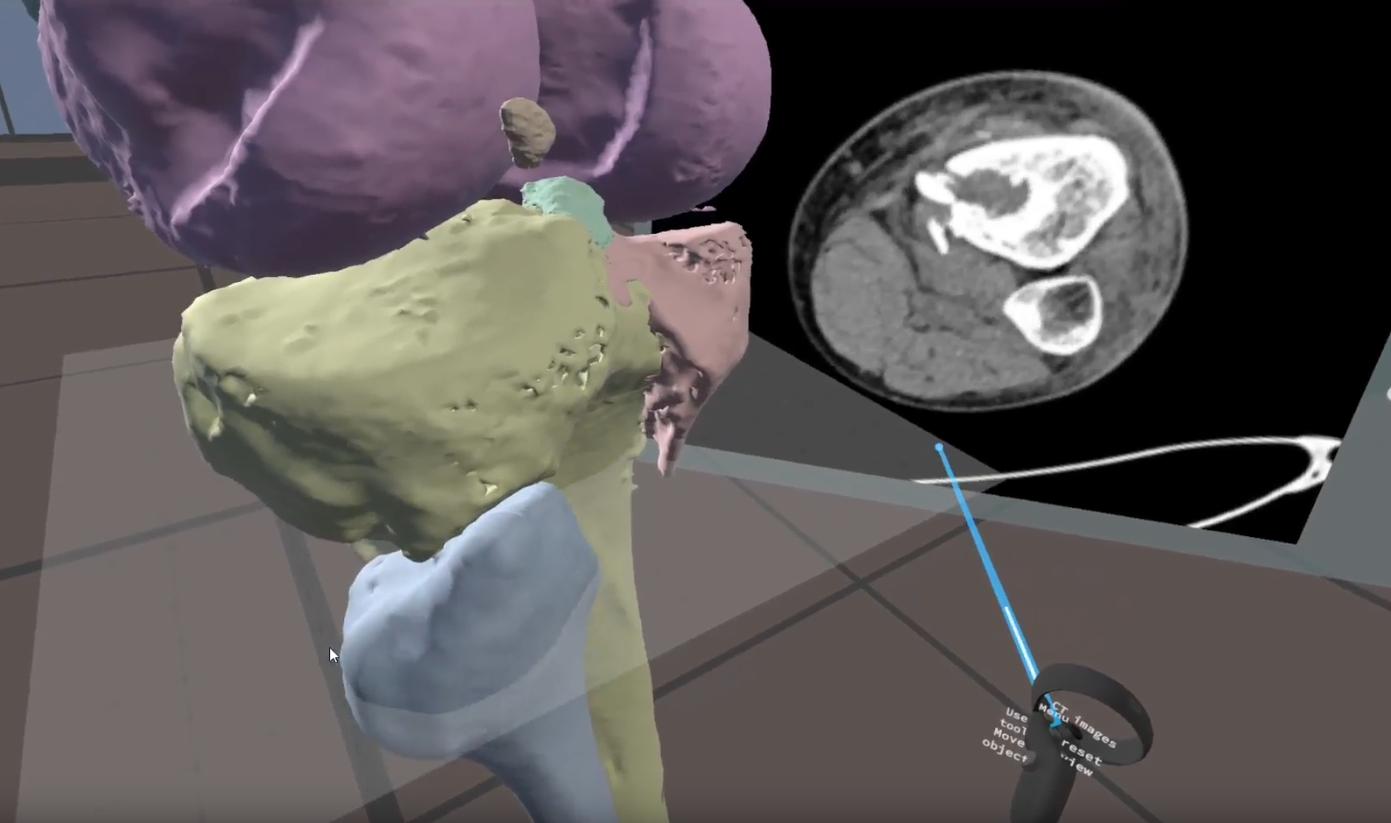
\includegraphics[height=120pt]{images/ctscan.png}}
	\hfill
  \caption{CT images}
  \small
  The user has moved the CT slice plane (transparent grey) to inspect the Tibia and Fibula (Shinbone/Calf Bone). The CT image on the right shows the CT scan of the two bones.
~\cite{mishra_virtual_2019}
\end{figure}

The slice number is calculated to convert between the selected height and the rendered CT image. This is done by getting the model's height and reading the y position of the selection plane. The height percentage of the plane is rounded down to the closest slice number, and that slice is shown.

\subsection{Rendering bone fragments}
In STL files all vertices are stored coordinates relative to the center, so by inserting all STL files at the same world space coordinate, the bone fragments will be placed correctly relative to each other. The STL files are exported to .obj files using blender and rendered with Unity.

--how the model is scaled

\subsubsection{Separating bone fragments}
Adding some form of manual splitting of meshes was considered. This would allow the user to split the model pieces into separate pieces further. This functionality would also make it possible to use models that are not split into pieces beforehand.
TODO: finish

An example open-source framework called Ezy-slice\cite{aryan} was tested.

\subsection{Alternative CT visualisation}
While rendering the selected slice as an image gave some understanding, there was still a disconnect between the model and the CT image. To improve upon this, I rendered the CT image at the exact position where it would intersect with the model.
This required removing the part of the model above/under the intersection plane, so it did not obscure the image. For this, I used a Unity Assetstore shader to view the cross-section of a mesh\cite{aldandarawy_unity_2019}.

This effect can be disturbing as the entire model is not visible. To allow for rendering the entire model, this rendering is a made optional. The option defaults to showing the entire model because it is easier to understand.
The toggle button is shown in the CT image options.

\begin{figure}[h!]
    \centering
	\subfloat[][]{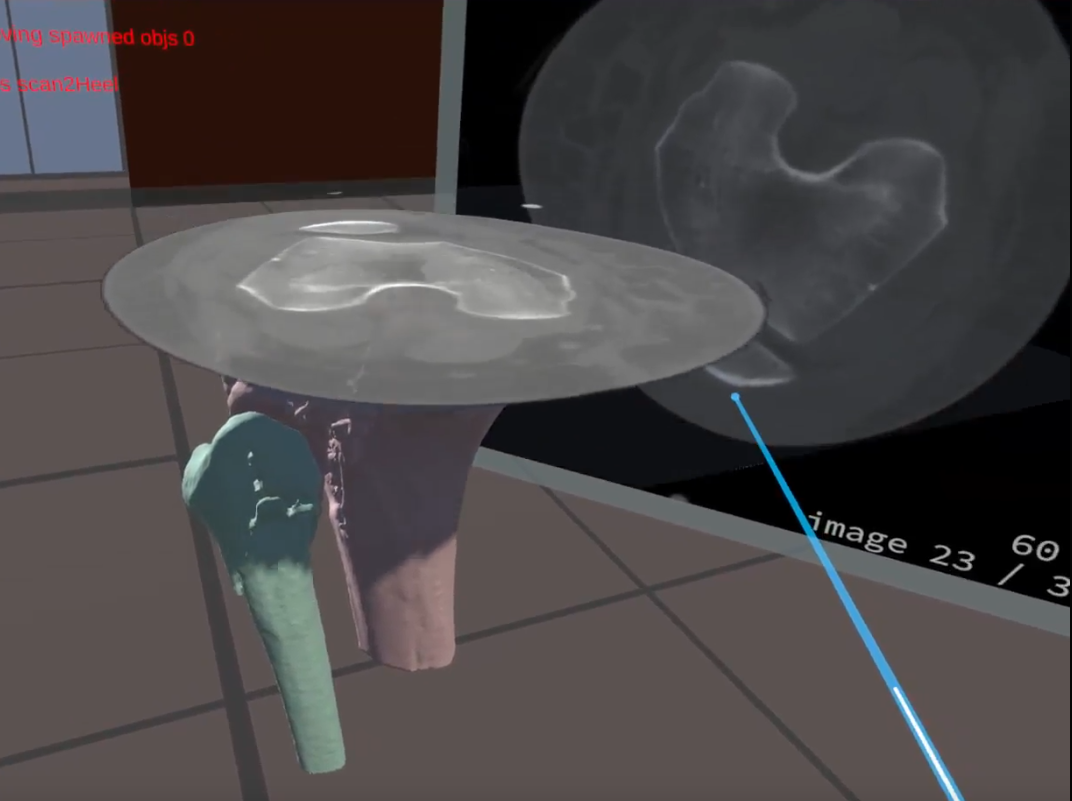
\includegraphics[height=120pt]{images/intersection.png}}
	\hfill
  \caption{CT intersection}
  \small
  The selected CT slice is shown both in 2D and as a overlay on top of model. Notice that the upper part of the model is not rendered.
\end{figure}

When overlaying the slice texture onto the intersection plane, the image will completely obscure the model when looking down at the image. This removes the point of overlaying the CT image, so the picture is created as partially transparent. When the texture is created, the grey value is used as input for calculating the transparency of the pixel. This results in most of the outside of the image being completely transparent.

\subsection{Implants}
The menu has a sub-menu for choosing what implant to add to the scene. It consists of a list with a description and a preview of the implant. Pressing a button will spawn the selected implant in front of the user, and can then be moved in the same way a model part can be moved.
To improve the surgeon's ability to line up screws and find what parts of the fracture is penetrated by the screw/object an outline is shown. This allows the user to see where an object is compared to any other parts, even if it is entirely obscured by the model. This is achieved by a shader using a depth buffer to only draw the outline when obscured by other meshes\cite{shader depth}.

\section{Performance}
Some performance guidelines are outlined by the Occulus developers for the Quest 1\cite{performance}.

The recommended triangle count is between 350k-500k triangles. The imported meshes can have a high vertex count and are reduced manually using Blender remeshing.
This could be automated, but this limit would be irrelevant using a headset using a GPU for dedicated rendering.


-mesh count and simplification\
-quest performance and other headsets performance
-performance data

\chapter{Use cases}\label{usecases}

\chapter{Analysis and assessment}\label{analysis and assessment}


\section{Evaluations}


\subsection{test 1}
date: 16 jan. 2022
This was the first test done with professional end users. The goal of the test was to figure out if any of the proposed usecases was relevant for the user. The test was performed by introducing the software, its potential usecases and a short introduction on how to use the VR controllers.
As both surgeons are very experienced with reading 2D CT images, they agreed that using 3D and VR to improve the understanding of fractures were minimal.

\begin{table}[ht]
\begin{tabular}{p{0.15\linewidth} |p{0.15\linewidth} |p{0.15\linewidth} | p{0.5\linewidth}}
Occupation         & Experience & proficiency with VR & comments                                                                                                                                \\hline
Orthopedic surgeon & 10+ years  & None                & The density of bone is important to know parts are solid enough for drilling. Also, some parts below the desnity threshold are missing. \\
Orthopedic surgeon & 10+ years  & None                & Smaller parts and bone fragments should be moveable to "reponere" bruddet.                                                              \\
                   &            &                     &
\end{tabular}
\end{table}

\section{compared to previous tools}

\section{compared to 3D printing}
-price
-time
-equal to or better performance

\chapter{Discussion}\label{Discussion}


\chapter{Conclusion} \label{Conclusion}

\chapter{Further Work} \label{Further Work}

\appendix
\chapter{Source code} \label{SourceCode}

The source code for the VR application is available at this URL: \url{https://github.com/tobias2912/VR-DICOM-viewer}.



%\bibliographystyle{splncs04}
%\bibliography{references}
\printbibliography

\end{document}
